\appendix
\chapter*{Appendices}
\addcontentsline{toc}{chapter}{Appendices}

\vspace{0.5cm}
\phantomsection
\label{appendix-a}
\section*{Appendix A: Sample Annotated Images}
This appendix contains a selection of annotated images used during the OCR dataset preparation phase. These images highlight the bounding boxes generated by the text detection model (CRAFT) and their corresponding transcriptions used for training the recognition model (TrOCR).

\begin{figure}[h]
    \centering
    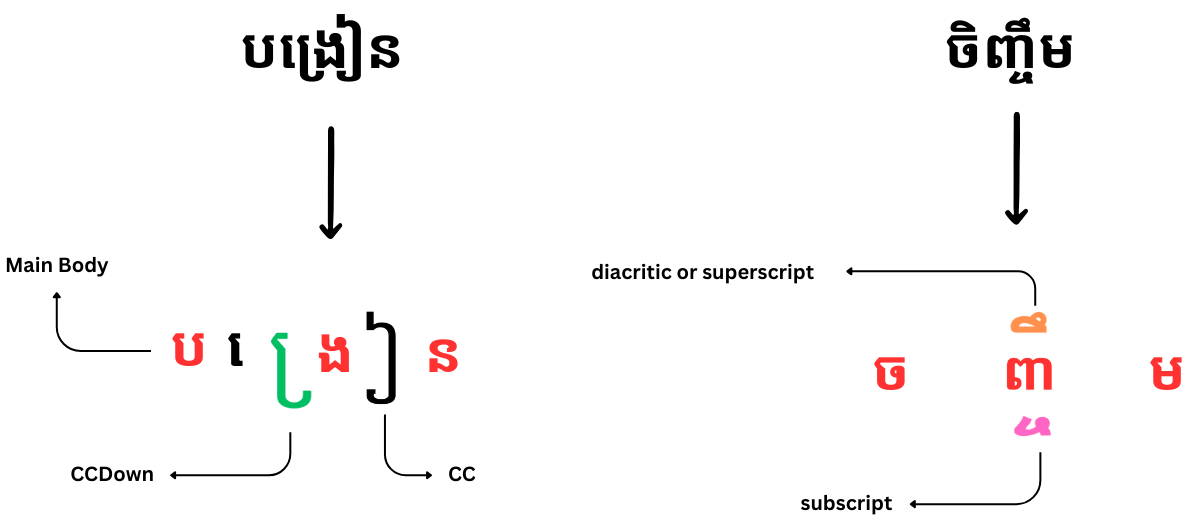
\includegraphics[width=0.8\textwidth]{figures/example_of_text_format.png}
    \caption{Example of text format showing different styles and layouts used in testing.}
\end{figure}

\clearpage
\phantomsection
\label{appendix-b}
\section*{Appendix B: List of Fonts Used}
This appendix lists the Khmer and Latin fonts used during synthetic data generation and model evaluation. Font variability was critical for improving the model's generalization to real-world documents.

\clearpage
\phantomsection
\label{appendix-c}
\section*{Appendix C: Code Snippets and Training Configuration}
This appendix includes key code snippets and hyperparameters used during model training.

\subsection*{Example TrOCR Training Configuration}
\begin{verbatim}
# Sample training configuration
model_args = {
    "model_name": "microsoft/trocr-base-stage1",
    "learning_rate": 5e-5,
    "warmup_steps": 500,
    "max_steps": 10000,
    "batch_size": 16,
    "max_length": 256
}

trainer = Trainer(
    model=model,
    args=TrainingArguments(**model_args),
    train_dataset=train_dataset,
    eval_dataset=val_dataset
)
\end{verbatim}

\subsection*{Example CRAFT Detection Parameters}
\begin{itemize}
    \item Text confidence threshold: 0.7
    \item Link confidence threshold: 0.4
    \item Input resolution: 1280x720
    \item Post-processing NMS threshold: 0.2
\end{itemize}

\clearpage
\phantomsection
\label{appendix-d}
\section*{Appendix D: Additional Evaluation Examples}
This appendix includes additional OCR results to showcase the model's behavior on varied layouts, font types, and Khmer-English mixed inputs.

\begin{figure}[h]
    \centering
    
\includegraphics[width=0.8\textwidth]{figures/example_of_sequential_text.png}
    \caption{Example showing sequential text processing and recognition capabilities.}
\end{figure}
